\chapter{Long Short-Term Memory}
\label{chapter:lstm}
\section{簡介}
\label{sec:LstmIntroduction}


在與序列資料有關的應用中,像是語音辨識、機器翻譯或是天氣與股市的預測,這些問題的輸入資料,往往會與前面或後面輸入的資料有關,因此不同的序列會直接影響輸出的結果。
但對於多層感知機(Multilayer Perceptron,MLP)來說,同樣的輸入通常會對應同樣的輸出,因此跟時間序列有關的問題,往往單用MLP是無法處理的。

而長短期記憶(Long Short-Term Memory,LSTM),為一種特殊的RNN,可以用來處理與序列資料有關的問題,圖\ref{fig:LstmUnit}為LSTM單一單元示意圖。LSTM的優勢在於透過Cell State這個關鍵元素,來保留過去的資訊,解決了Simple RNN 無法記住長期記憶的問題。更透過Forget Gate、Input Gate及Output Gate,使其能丢棄或保留過去的資訊。圖\ref{fig:LstmArchiture}為LSTM結構示意圖,可以看到每個單元會得到一個新的輸⼊ \(x_t\),並透過上一層運算完的Cell State 與 Hiden State 來,計算新的輸出、Hinden State 與 Cell State,並傳到下一層。

\begin{figure}[h]
	\centering
	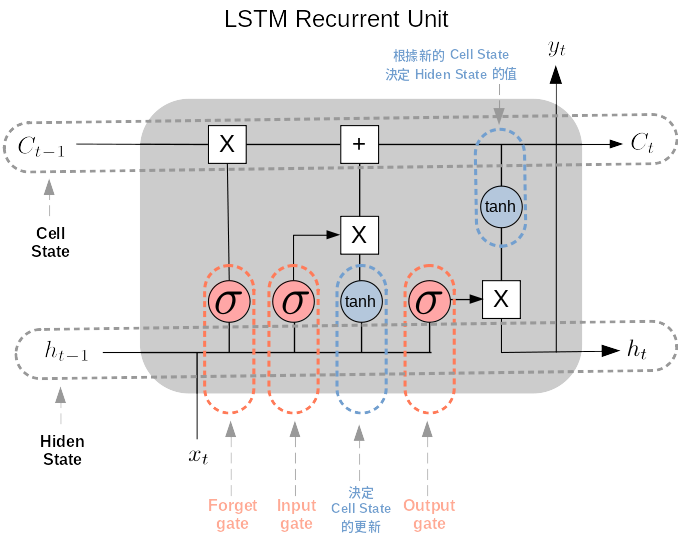
\includegraphics[width=10cm]{./pic/qpImeDw4.png}
	\caption{LSTM單一單元示意圖}
	\label{fig:LstmUnit}
\end{figure}


\begin{figure}[h]
	\centering
	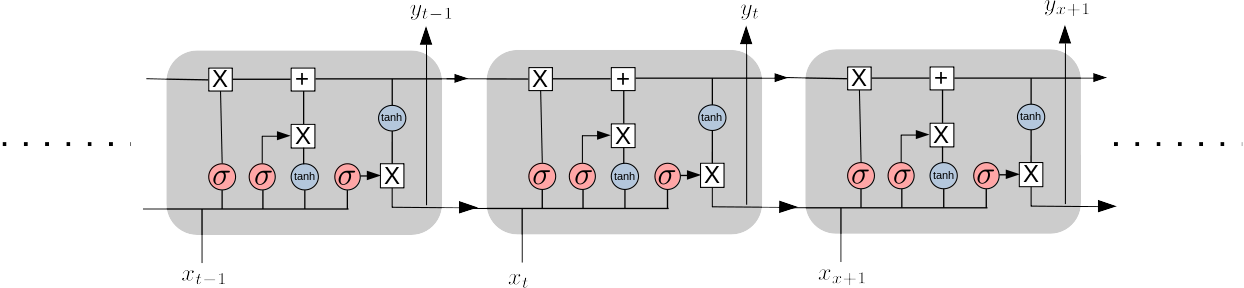
\includegraphics[height=3.5cm]{./pic/rDEsxEUS.png}
	\caption{LSTM結構示意圖}
	\label{fig:LstmArchiture}
\end{figure}


\newpage

\section{LSTM內部運作原理}

前一節提到,LSTM會透過不同的Gate來調節每個單元要丢棄或保留的訊息。LSTM是一個相對複雜的模型,以下會詳細介紹每個Gate的運作機制,以及Cell State 與 Hiden State 是如何更新的。



\subsection{Forget Gate}

LSTM的Forget Gate,故名思意就是決定丟棄多少程度的Cell State資訊,這個Gate的輸出為介於0到1的值,0表示「完全丟棄」,1表示「完全保留」。

\begin{itemize}
	\item 
		\(x_t\),表示第t個輸入向量,是一個具有\(n\) 代表向量的特徵數,在圖 \ref{fig:ForgetGateCalculate}中\(n = 3\) 

	\item 
		\(h_{t-1}\),為前一層的輸出結果,是一個 \(k \times 1\) 向量,\(k\)由自行決定,在圖 \ref{fig:ForgetGateCalculate}中\(k = 4\) 

	\item 
		\(W_f\),為forget gate的權重,是一個 \(k \times (k+n)\)的矩陣。

	\item 
		\(b_f\),為forget gate的偏移值,是一個 \(k \times (k+n)\)的矩陣。
\end{itemize}



\begin{figure}[H]
	\centering
	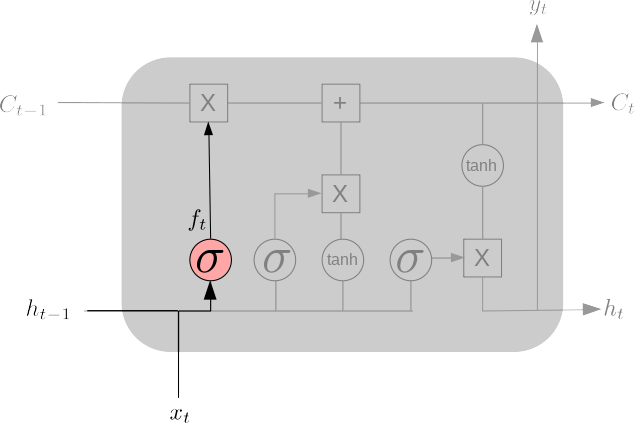
\includegraphics[width=10cm]{./pic/DR88VjoI.png}
	\caption{Forget Gate的流程}
	\label{fig:ForgetGate}
\end{figure}

\begin{figure}[H]
	\centering
	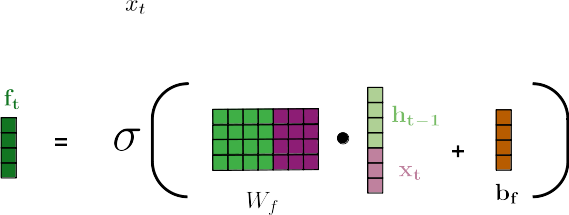
\includegraphics[width=9cm]{./pic/1hRe7Dz4.png}
	\caption{\(\mathbf{f_t}\)的運算示意圖}
	\label{fig:ForgetGateCalculate}
\end{figure}

\begin{equation}
	\label{eqn:ForgetGateCalculate}
	f_t = \sigma(W_f\cdot[h_{t-1},x_t]+b_f)
\end{equation}


\subsection{Input Gate}

在這個階段中,會決定新的訊息是否儲存Cell State的中。其中 Input Gate 會決定新的資訊更新的程度,而 \(C_t'\)則會決定要被更新的值。以下為相關的參數說明:


\begin{itemize}

	\item 
		\(W_i\),為Input gate的權重,是一個 \(k \times (k+n)\)的矩陣。

	\item 
		\(b_i\),為Input gate的偏移值,是一個 \(k \times 1\)的向量。

	\item 
		\(W_{c'}\),為決定\(C_t'\)的權重,是一個 \(k \times (k+n)\)的矩陣。

	\item 
		\(b_{c'}\),為決定\(C_t'\)的偏移值,是一個 \(k \times 1\)的向量。

\end{itemize}


\begin{figure}[H]
	\centering
	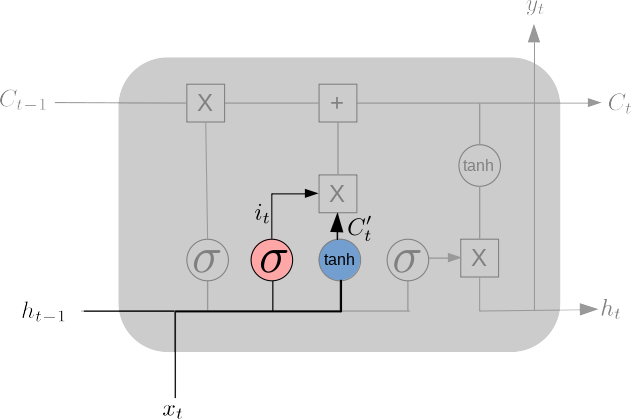
\includegraphics[width=10cm]{./pic/Htq3Iron.png}
	\caption{Input Gate的流程}
	\label{fig:InputGate}
\end{figure}


\begin{figure}[H]
	\centering
	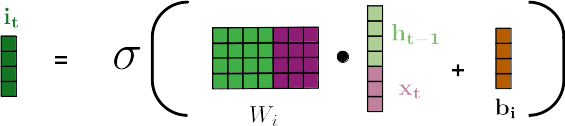
\includegraphics[width=9cm]{./pic/P11XgmjT.png}
	\caption{\(\mathbf{i_t}\) 的運算示意圖}
	\label{fig:InputGateCaculate}
\end{figure}

\begin{equation}
	\label{eqn:InputGateCalculate}
	i_t = \sigma(W_i\cdot[h_{t-1},x_t]+b_i)
\end{equation}

\begin{figure}[H]
	\centering
	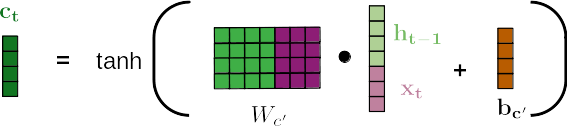
\includegraphics[width=9cm]{./pic/EI5hsLBg.png}
	\caption{\(\mathbf{C_t}\) 的運算示意圖}
	\label{fig:InputCalculate}
\end{figure}


\begin{equation}
	\label{eqn:InputCalculate}
	C_t' = tanh(W_i\cdot[h_{t-1},x_t]+b_i)
\end{equation}

\subsection{Cell State的更新}

Cell State的更新會根據,Forget Gate、Input Gate與 \(C_t'\)決定過去的資訊要被更新,或是被丟棄,進而產生新的。從圖\ref{fig:CellStateUpdateCaculate}可以觀察到,會將 \(C_{t-1}\)與 \(f_t\)行內積,決定舊的資訊要保留多少;然後再將\(C_t'\)與 \(i_t\)進行內積,決定要更新的資訊。最後相加得到新的\(C_t\)。

\begin{figure}[H]
	\centering
	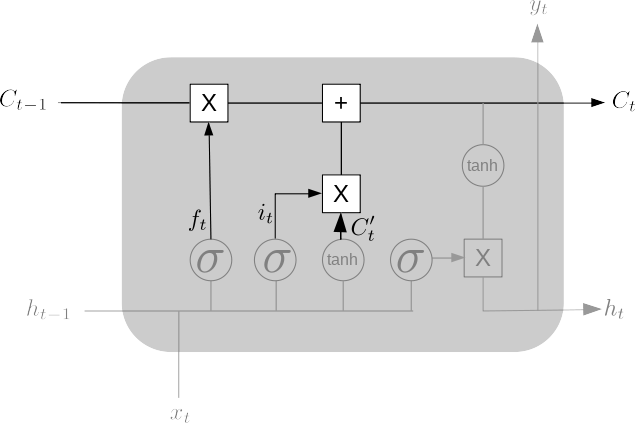
\includegraphics[width=10cm]{./pic/rQqms2xi.png}
	\caption{Cell State的更新的流程}
	\label{fig:CellStateUpdate}
\end{figure}


\begin{figure}[H]
	\centering
	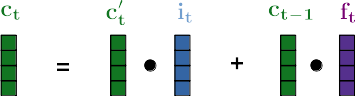
\includegraphics[width=9cm]{./pic/Qff4EdKi.png}
	\caption{\(\mathbf{c_t}\) 的運算示意圖}
	\label{fig:CellStateUpdateCaculate}
\end{figure}

\begin{equation}
	\label{eqn:InputCalculate}
	C_t' = c_t'\cdot i_t + c_{t-1}\cdot f_t 
\end{equation}



\subsection{Output Gate}

Output Gate會先決定更新後的Cell State輸出程度 \(o_t\) ,接著\(C_t\)會先進過tanh函數,其輸出值會介於-1到1之間,最後會與\(o_t\)內積,得到新的輸出結果 \(h_t\) 。

\begin{itemize}

	\item 
		\(W_o\),為Output gate的權重,是一個 \(k \times (k+n)\)的矩陣。

	\item 
		\(b_o\),為Output gate的偏移值,是一個 \(k \times 1\)的向量。

\end{itemize}

\begin{figure}[H]
	\centering
	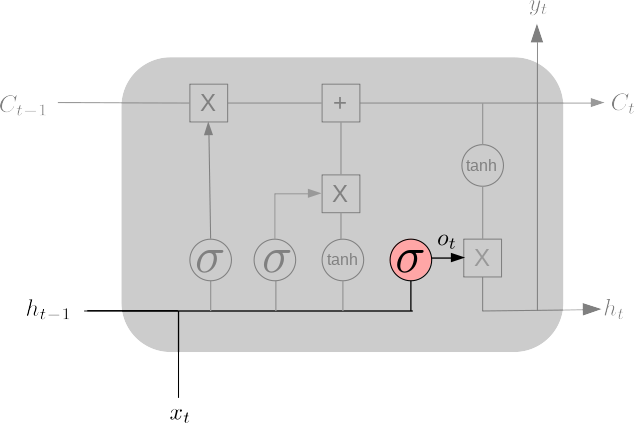
\includegraphics[width=10cm]{./pic/e9dbHfq4.png}
	\caption{Output Gate的流程}
	\label{fig:OutputGate}
\end{figure}


\begin{figure}[H]
	\centering
	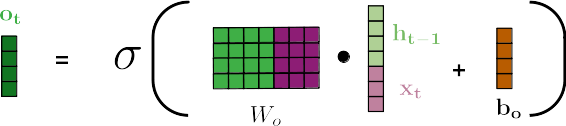
\includegraphics[width=9cm]{./pic/bcjXoMZk.png}
	\caption{\(\mathbf{o_t}\) 的運算示意圖}
	\label{fig:OutputGateCalculate}
\end{figure}

\begin{equation}
	\label{eqn:OutputGateCalculate}
	o_t = \sigma(W_o\cdot[h_{t-1},x_t]+b_o)
\end{equation}

\begin{figure}[H]
	\centering
	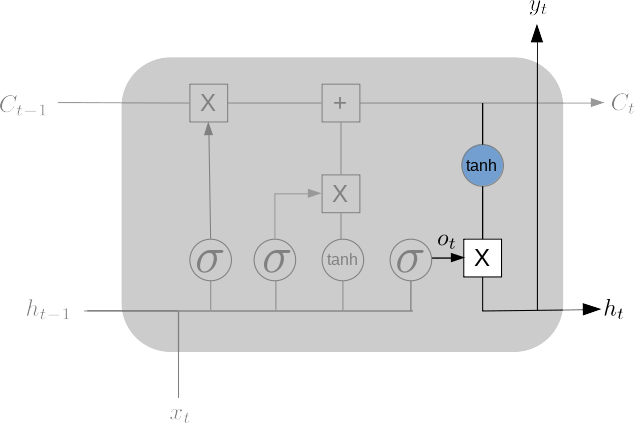
\includegraphics[width=10cm]{./pic/evwQIqAz.png}
	\caption{Hiden State的更流程}
	\label{fig:HidenStateUpdate}
\end{figure}


\begin{figure}[H]
	\centering
	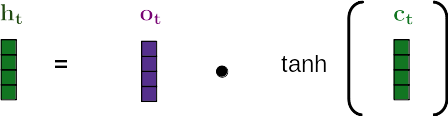
\includegraphics[width=9cm]{./pic/vo6a2bAS.png}
	\caption{\(\mathbf{h_t}\) 的運算示意圖}
	\label{fig:HidenStateUpdateCaculate}
\end{figure}


\begin{equation}
	\label{eqn:InputCalculate}
	h_t = o_t \cdot tanh(c_t) 
\end{equation}



\section {結論}

雖然LSTM的模型相較其他的模型來說複雜許多,也因為它多了Gate的機制,所以模型的參數會是其他模型的四倍,因此在模型訓練時,所需要的訓練時間會比較長。但僅管如此,LSTM所帶來的優點,除了能夠應用於時間序列的資料上,更能夠記憶更長的時間序列。因此在與序列資料有關的應用中,幾乎都會使用LSTM來進行模型訓練。




